\documentclass[9pt]{beamer}
\usepackage[utf8]{inputenc}
\usepackage{txfonts}
\usepackage[english]{babel}
\usepackage{xcolor}
\usetheme{AnnArbor}
\usecolortheme{beaver}

\setbeamertemplate{headline}{}
% \setbeamertemplate{frametitle}{\insertframetitle}
\setbeamertemplate{navigation symbols}{}

\setbeamertemplate{itemize item}{\scriptsize\raise1.25pt\hbox{\donotcoloroutermaths$\blacktriangleright$}}
\setbeamertemplate{itemize subitem}{\tiny\raise1.5pt\hbox{\donotcoloroutermaths$\blacktriangleright$}}
\setbeamertemplate{itemize subsubitem}{\tiny\raise1.5pt\hbox{\donotcoloroutermaths$\blacktriangleright$}}
\setbeamertemplate{enumerate item}{\insertenumlabel.}
\setbeamertemplate{enumerate subitem}{\insertenumlabel.\insertsubenumlabel}
\setbeamertemplate{enumerate subsubitem}{\insertenumlabel.\insertsubenumlabel.\insertsubsubenumlabel}
\setbeamertemplate{enumerate mini template}{\insertenumlabel}

% \setbeamertemplate{itemize items}[square]
% \setbeamertemplate{items}[square]



\newcommand{\bluemph}[1]{\structure{\emph{#1}}}
\newcommand{\redemph}[1]{\alert{\emph{#1}}}
\newcommand{\bluebf}[1]{\structure{\textbf{#1}}}
\newcommand{\redbf}[1]{\alert{\textbf{#1}}}

\newcommand\denote[1]{\llbracket #1 \rrbracket}
\newcommand\fesi{Fe-Si}

%  Structure
\newenvironment{remark}{\footnotesize \begin{description}\item[\emph{Remark}:]}{\end{description}}

\title{Package manager for Coq}
\author{Thomas Braibant}
\institute[Inria]{Inria}
\date[11/2013]{11/2013}

\setbeamercovered{transparent}
%\setbeamerfont{frametitle}{size={\normalsize}}

% \usepackage[T1]{fontenc}
\usepackage{amsmath}
\usepackage{amssymb}
\usepackage{amsthm}
\usepackage{mathpartir}

\usepackage{listings}
\usepackage{graphicx}
\definecolor{ltblue}{rgb}{0,0.4,0.4}
\definecolor{dkblue}{rgb}{0,0.1,0.6}
\definecolor{dkgreen}{rgb}{0,0.4,0}
\definecolor{dkviolet}{rgb}{0.3,0,0.5}
\definecolor{dkred}{rgb}{0.5,0,0}
\usepackage{lstcoq}
\usepackage{lstocaml}
\usepackage{tikz}

\begin{document}
% \newcommand \blue[1]{{\color{red!80!black}{#1}}}
\newcommand \orange[1]{{\color{orange}{#1}}}
% \newcommand \red[1]{{\color{red}{#1}}}
% \newcommand \grey[1]{{\color{gray}{#1}}}
% \newcommand \green[1]{{\color{violet}{#1}}}
% \newcommand \white[1]{{\color{white}{#1}}}

\newcommand\parenthesis[1] {
  \begin{flushright}
    {\scriptsize \redemph{{{{ #1}}}}}
  \end{flushright}

}

\newcommand\plan[2]
{
\begin{frame}[plain]
  \begin{center}
    {\Huge  \sc #1} \\

    \vspace{1cm}

    #2
\end{center}
\end{frame}
}

\plan{Package managing for Coq}{}

\begin{frame}[plain]
  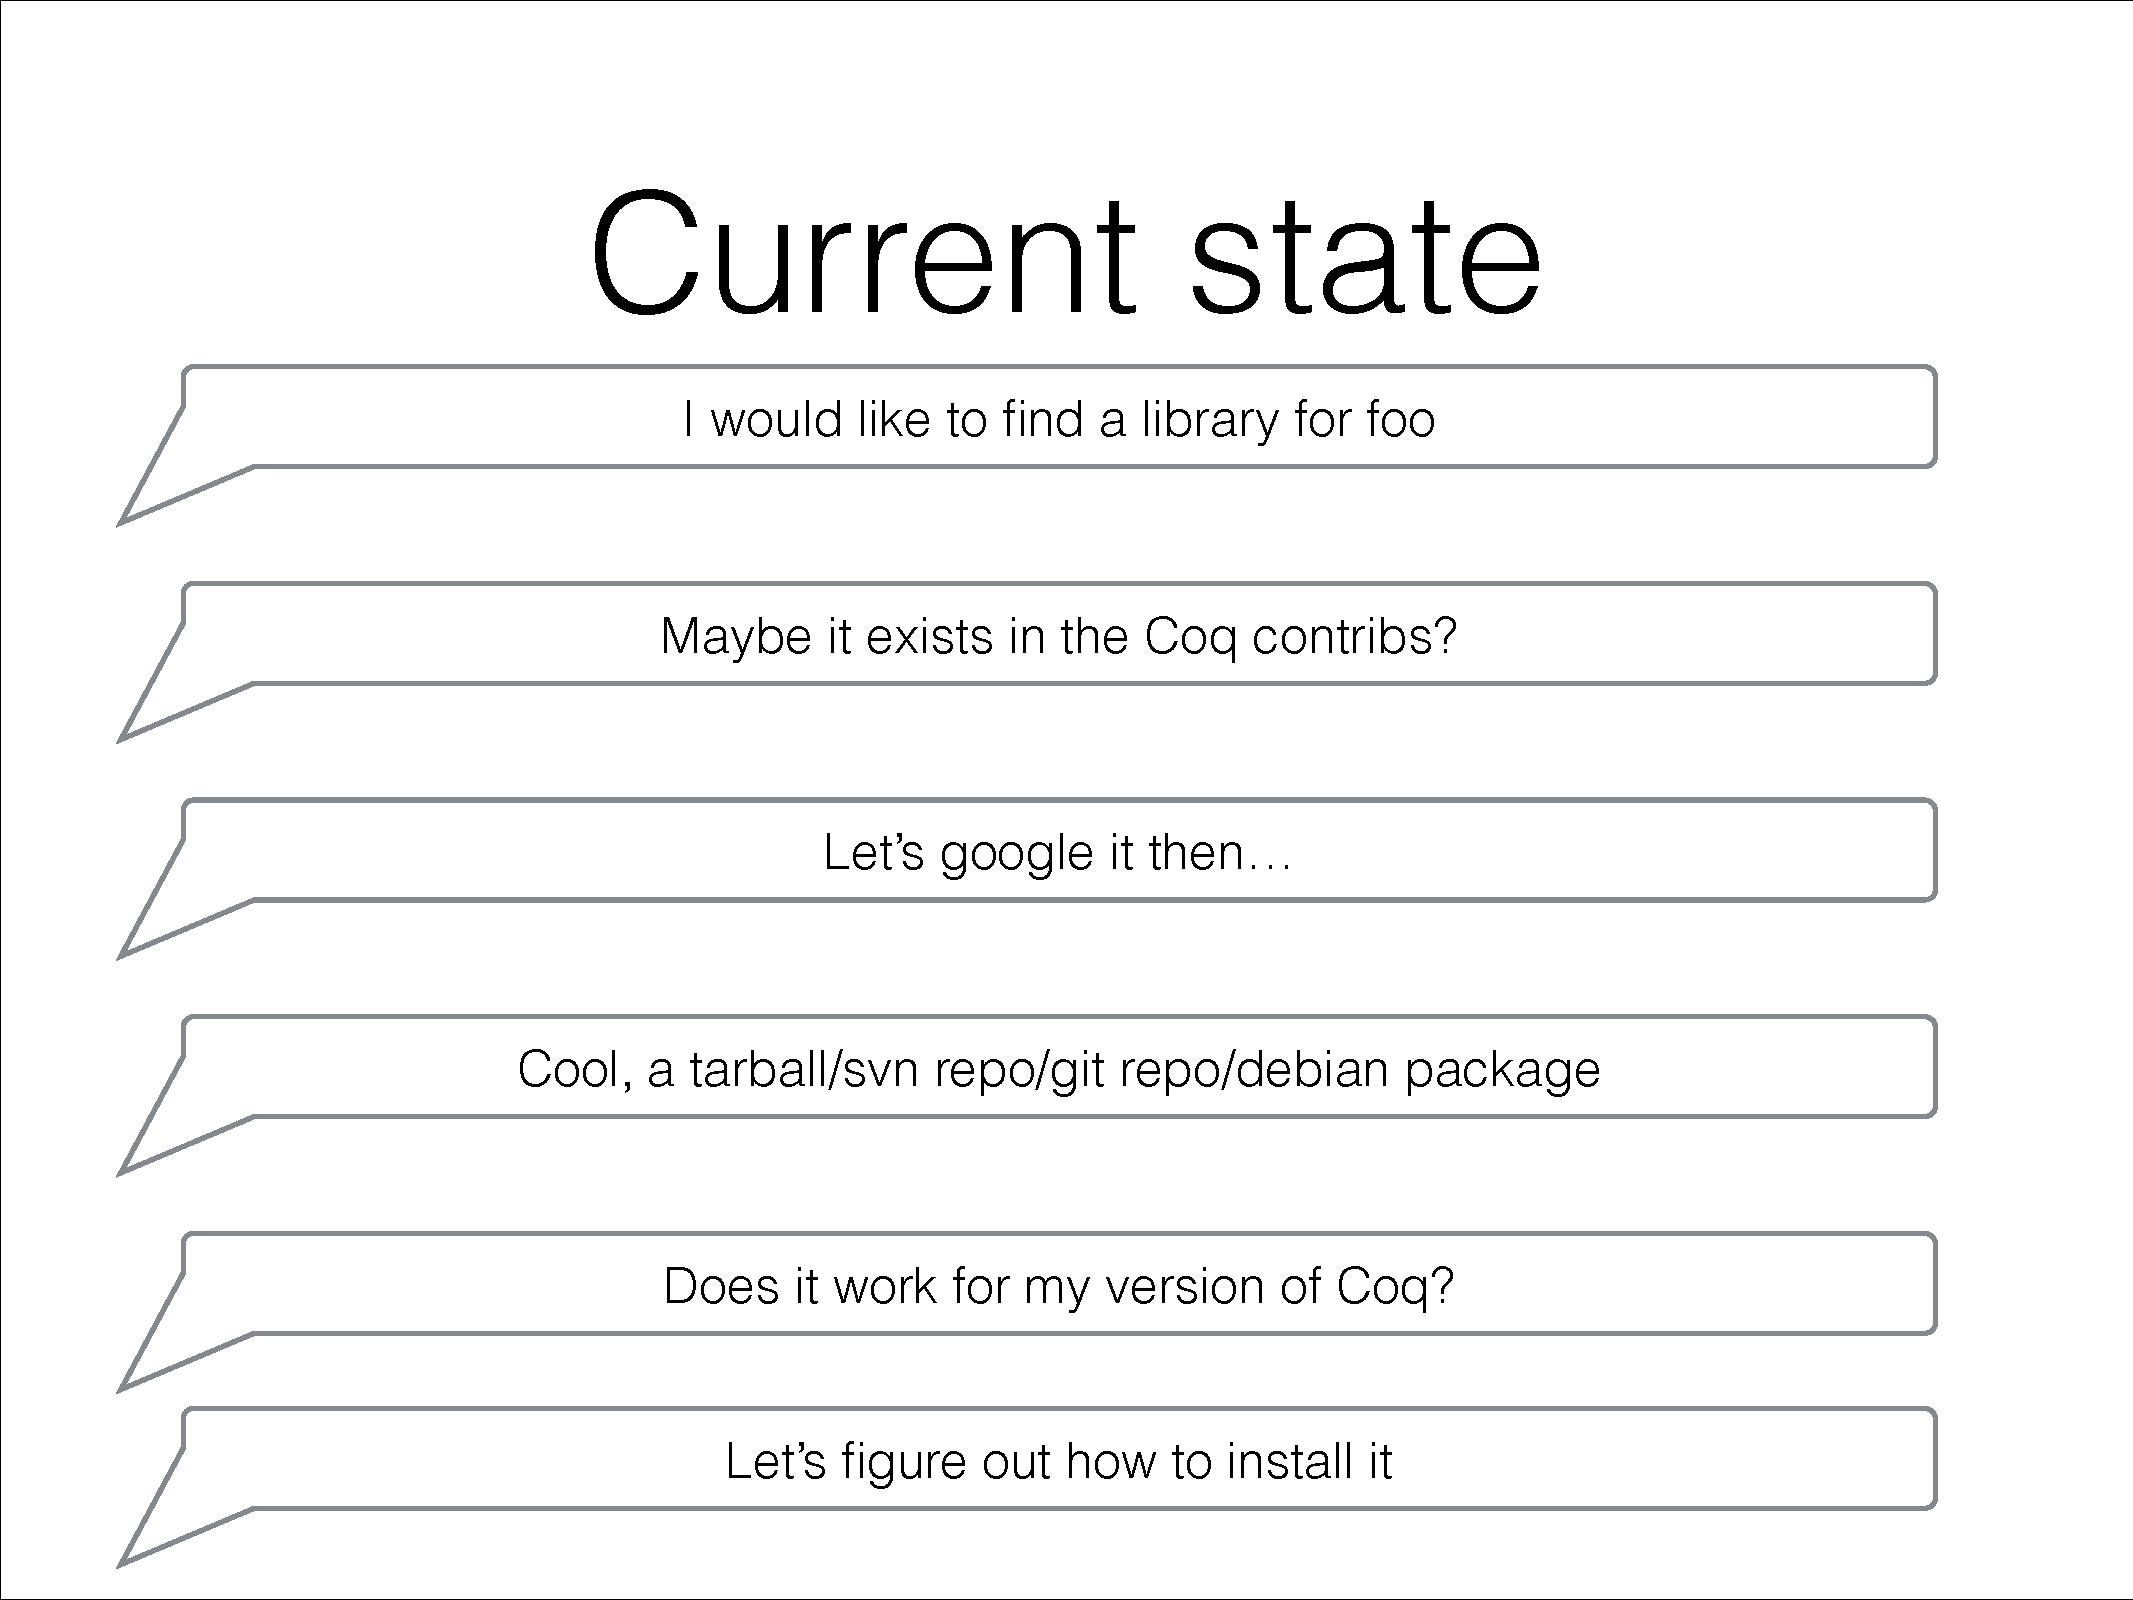
\includegraphics[width=\linewidth]{figs/current-state.pdf}
\end{frame}

\begin{frame}{Problems}
  \begin{itemize}
  \item No centralized repository of packages
  \item No unified build system
  \item Monolithic packages (e.g. ssreflect, CompCert, CoLoR, \dots)
  \item No easy way to have multiple Coq installs \\
    \parenthesis{symlink, make install, and so on}
  \end{itemize}
\end{frame}


\plan{Plan A}{\textbf{Implement a package manager from scratch}}

\begin{frame}
  \frametitle{Plan A}
  \begin{itemize}
  \item Time consuming
  \item Error prone
  \item Not ``science''
  \end{itemize}
\end{frame}

\plan{Plan B}{\textbf{Forking an exisiting package manager: opam}}

\begin{frame}
  \title{Forking opam}
  \begin{itemize}
  \item opam knows of (ocaml) \alert{'compilers'} and 'packages'
    \pause
  \item search and replace:
    \begin{itemize}
    \item opam with cpam
    \item ocaml with coq
    \end{itemize}
    \pause
  \item What if the OCaml version of the system changes?
  \item What about dependencies between Coq packages (plugins) and OCaml  packages?
  \end{itemize}
\end{frame}


\plan{Plan C}{\textbf{Modify an existing package manager: opam}}

\begin{frame}[fragile]
  \frametitle{Opam primer}
  \begin{itemize}
  \item Each 'state' is stored in one {\verb!$opam/$switch!}
  \item Each 'state' has its own OCaml compiler and set of packages
  \item {\tt opam switch 4.01.0} will:
    \begin{itemize}
    \item create a new switch if needed
    \item install the ocaml compiler version 4.01.0
      \pause
    \item update the configuration env. if the switch already exists
    \end{itemize}
    \pause
  \item {\tt opam install foobar} will:
    \begin{itemize}
    \item lookup for the available versions of package {\tt foobar};
    \item select the highest version available for the current compiler; 
    \item update other packages if needed
    \end{itemize}
  \end{itemize}
  
  \pause
  
  \begin{center}
    Powerful system to resolve dependencies between packages
  \end{center}
\end{frame}

\begin{frame}
  \frametitle{Prototype}
  
  New commands for opam. 
  \begin{itemize}
  \item {\tt opam coq install coq.8.4.2} will:
    \begin{itemize}
    \item create a new opam switch named {\tt myocamlversion--coq.8.4.2}
    \item install Coq 8.4pl2 in this switch (with its dependency on camlp5)
    \end{itemize}
    \pause
  \item {\tt opam coq switch coq.HoTT} will:
    \begin{itemize}
    \item browse the existing switches to find one with Coq HoTT; 
      \pause
    \item if there is exactly one, will 'switch' to it;
    \item if there is more than one, will tell the user to select one;
    \item if there is none, will install one (with a fresh a OCaml compiler)
    \end{itemize}
    \pause
  \item {\tt opam coq list} will: 
    \begin{itemize}
    \item show the available installs of Coq (similiar to {\tt opam switch})
    \end{itemize}
  \end{itemize}
\end{frame}

\begin{frame}[fragile]
  \frametitle{One word}
  
  \begin{itemize}
  \item Coq is a \alert{regular} opam package
  \item Coq packages are \alert{regular} opam packages
  \item The front-end uses \alert{regular} opam switches
  \item The front-end uses \alert{regular} opam 'pins' (to pin the installed version of Coq)
  \end{itemize}
  
\end{frame}

\begin{frame}[fragile]
  \frametitle{Coq 8.4pl2}

\lstset{basicstyle=\footnotesize, frame=single}

\begin{lstlisting}
archive: "http://coq.inria.fr/distrib/V8.4pl2/files/coq-8.4pl2.tar.gz"    
\end{lstlisting}

  \begin{columns}
\column{0.45 \linewidth}

  \begin{lstlisting}
opam-version: "1.1"
patches: ["configure.patch"]
build: [
  [ "./configure" 
     "-configdir" "%{lib}%/coq/config"
     "-mandir" "%{man}%"
     "-docdir" "%{doc}%"
     "--prefix" "%{prefix}%"
     "--usecamlp5"
     "--coqide" "no"
#     "-opt"
  ]
  [ "make" "-j4" "world"]
  [ "make" "install"]
]
depends: ["camlp5"]    
  \end{lstlisting}
    \column{0.35\linewidth}
    \begin{itemize}
    \item camlp5 by default
    \item opt compilers?
    \item set of patch
    \end{itemize}
  \end{columns}
\end{frame}

\begin{frame}[fragile]
  \frametitle{Coq 8.4pl2+mtac}
  \begin{columns}
\column{0.4 \linewidth}
\lstset{basicstyle=\footnotesize}
  \begin{lstlisting}
opam-version: "1.1"
patches: ["configure.patch" "mtac-1.1.patch"]
build: [
  [ "./configure" 
     "-configdir" "%{lib}%/coq/config"
     "-mandir" "%{man}%"
     "-docdir" "%{doc}%"
     "--prefix" "%{prefix}%"
     "--usecamlp5"
     "--coqide" "no"
#     "-opt"
  ]
  [ "make" "-j4" "world"]
  [ "make" "install"]
]
depends: ["camlp5"]    
  \end{lstlisting}
    \column{0.35\linewidth}
    \begin{itemize}
      \item One line of difference!
    \end{itemize}
  \end{columns}
\end{frame}

\begin{frame}[fragile]
  \frametitle{ssreflect}

\lstset{basicstyle=\footnotesize}

  \begin{lstlisting}
archive:"http://ssr.msr-inria.inria.fr/FTP/ssreflect-1.5rc1.tar.gz"
checksum: "c08130242ea2cfd1cb4ae8754fa411fe"
  \end{lstlisting}
  \begin{columns}
\column{0.4 \linewidth}
  \begin{lstlisting}
opam-version: "1.1" 
maintainer: "thomas.braibant@gmail.com"
build: [
  [make]
  [make "install"]
]
depends: [ "coq" { >= "8.4.2"}]
  \end{lstlisting}
    \column{0.35\linewidth}
    \begin{itemize}
      \item Version constraints
    \end{itemize}
  \end{columns}
\pause
\begin{center}
  In practice, in Coq, all package constraints should use 'equals'!
\end{center}
\end{frame}

\begin{frame}
  \frametitle{Current state}
  \begin{center}
    \begin{tabular}{l}
      HoTT.stable	\\
      aac\_tactics.0.4	 \\
      compcert.2.0+ia32-linux \\
      containers.2010	 \\
      coq.8.4.2+mtac	\\
      coq.8.4.2	\\
      coq.8.4.3dev	\\
      coq.8.5dev	\\
      coq.HoTT+stable	\\
      counting.2010	\\
      cybele.1.2dev	\\
      ergo.2010	        \\
      flocq.2.2.0	\\
      interval.0.16.1	\\
      mathcomp.1.5	\\
      ssreflect.1.5  
    \end{tabular}
  \end{center}
  \parenthesis{Various versions of the same package.}
\end{frame}

\begin{frame}
  \frametitle{Questions}
  
  \begin{itemize}
  \item Examples of \alert{unfinished} packages
    \begin{itemize}
    \item Ergo (from contribs) does not compile out of the box!
    \item CoLoR has no install target (easy)
    \end{itemize}
    \pause
  \item Configuration options? (one of a kind problem for CompCert)
    \begin{itemize}
    \item One package per compcert set of options?
    \end{itemize}
    \pause
  \item Semantic versioning? ({\tt semver.org}) \\
    \begin{quote}
      Given a version number MAJOR.MINOR.PATCH+tag, increment the:
      \begin{enumerate}
      \item MAJOR version when you make incompatible API changes;
      \item MINOR version when you add functionality in a
        backwards-compatible manner;
      \item PATCH version when you make backwards-compatible bug
        fixes.
      \end{enumerate}
    \end{quote}
    \pause
  \item How to deal with git branches as releases? (HoTT)
  \item camlp5/camlp4?
  \item coq\_makefile, uninstall targets?
  \item Merge {\tt user-contribs}, {\tt theories}?
  \item Good uses of {\tt -R}, {\tt -I}?
  \end{itemize}
\end{frame}

\begin{frame}
  \frametitle {Perspectives}

  \begin{itemize}
  \item Fine grained packages 
  \item Stripped down Coq (libraries and plugins as separate packages)
  \item Download statistics (how much something is used)
  \item Opam2Web (to list packages)
  \item Ocamlot (continuous integration/test infrastructure)
  \item SDK for Windows, OS X, GNU/Linux (Vagrant?)
  \item Use libraries in Coq (pprint, framaC/unmarshal, ancient, persistent arrays, ...)
  \item Use cutting-edge OCaml (gadts, ephemerons, ...)
  \item Multiple repos of Coq packages
  \end{itemize}
\end{frame}

\begin{frame}{URLs}
  \begin{itemize}
  \item \texttt{https://github.com/braibant/opam}
  \item \texttt{https://github.com/braibant/opam-coq-repo}
  \end{itemize}  

  \parenthesis{Pull-requests welcome}

  \parenthesis{Move it to coq.inria.fr?}
\end{frame}
\plan{Plan D}{\textbf{Package Coq specific commands as an opam package} 

  \vspace{2em}
  \parenthesis{On my todo-list}  
}


\plan{TL; DR}{\textbf{    
\begin{tabular}{l}
      OPAM \\
      ONLY\\
      DOES \\
      \alert{EVERYTHING}
    \end{tabular}
}    

\tiny{thanks OCamlPro}
}

\plan{One more thing}{
  \textbf{Survey about Coq}

  \vspace{1em}

  \begin{itemize}
  \item Know the users (researchers, teachers, students, numbers)
  \item Know what they do (math, pl, production)
  \item Know how they work (ide, how much time, tactics)
  \item Know what library/plugin/contrib they use (are contribs used)
  \item Know what they find important (doc, perf, backward compatibility, new features)
  \item Guide development
  \end{itemize}
}


\end{document}
